\subsection{NVFP4 Training}
\label{subsec:nvfp4}

We demonstrate stable and accurate pretraining on a hybrid Mamba-MoE architecture for up to 25T tokens using the NVFP4 number format. Weight, activation, and gradient tensors are quantized to NVFP4 which enables use of NVFP4 GEMMs in fprop, dgrad, and wgrad. On GB300, peak FP4 throughput is 3$\times$ higher than FP8 throughput~\citep{nvidia2025blackwellultra}. Prior work in NVFP4 pretraining ~\citep{nvidia2025pretraininglargelanguagemodels} simulated NVFP4 numerics through quantize-dequantize functions around BF16 GEMMs. This work uses native NVFP4 GEMMs, leveraging cuBLAS's backend for Transformer Engine.

The NVFP4 format features: fine-grained (16 element) micro-block scaling, block scaling factors with E4M3 format, a second-level FP32 global scale, and the E2M1 element format. We utilize two-dimensional (2D) block scaling for weight quantization, Random Hadamard Transforms (RHTs) on inputs to wgrad, and stochastic rounding on gradients. We kept the last 15\% of the network in high precision to maintain stability. % We used amax-based scaling.

Super and Ultra models employ the Latent-MoE architecture and MTP. We kept latent projections in BF16 as its impact to step-time is minimal. We also keep MTP layers in BF16 due to their positioning at the end of the network and to preserve MTP capabilities.

The Nemotron 3 family of models features a small ratio of attention to Mamba-2 layers, and each attention layer uses GQA with only 2 KV heads. To maintain the fidelity of these few attention layers, we kept the QKV and attention projections in BF16. We observed that Mamba output projection layers have high flushes to zero (up to 40\% on Nano) when quantized to NVFP4. To prevent loss of information, we keep these layers in MXFP8. Figure~\ref{fig:nanov3_loss_diff_nvfp4} shows that combining both modifications resulted in a recipe that improved both train and validation loss (green) compared to keeping these layers in low precision (blue).

\begin{figure}[]
    \centering
    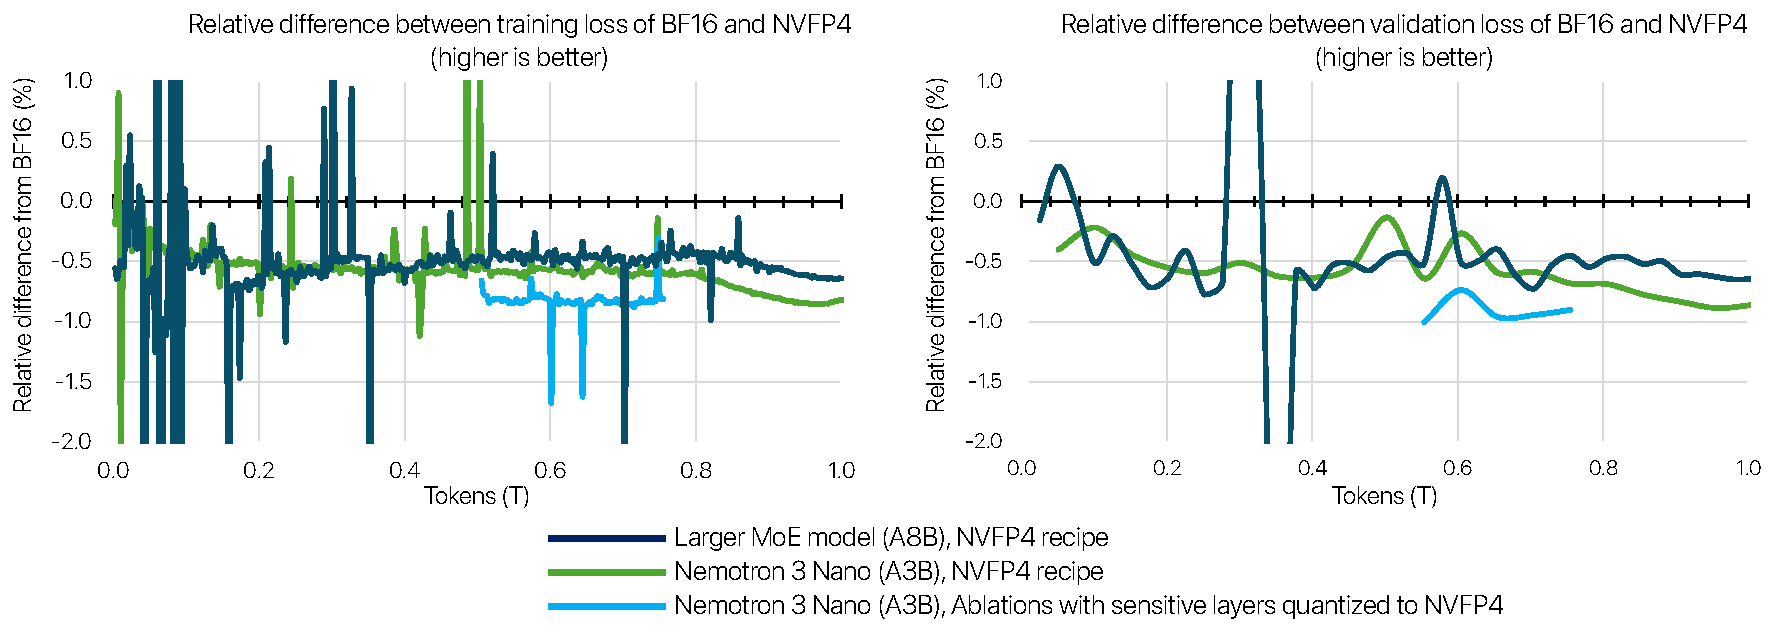
\includegraphics[width=\textwidth]{figures/relative_loss_diffs_nvfp4.pdf}
    \caption{Relative difference in train loss (left) and validation loss (right) between models trained with NVFP4 and BF16, shown at two model scales: Nemotron 3 Nano (A3B) and the larger MoE model (A8B). Loss gaps decrease as model size increases (A3B $\to$ A8B). Recipe ablation on Nemotron 3 Nano started from Nemotron 3 NVFP4 checkpoint at 500B tokens, then quantizes sensitive layers (Mamba Output, QKV, and Attention projections) to NVFP4, highlighting the importance of keeping these layers in high precision.  
    }
    \label{fig:nanov3_loss_diff_nvfp4}
\end{figure}


\begin{figure}[]
    \centering
    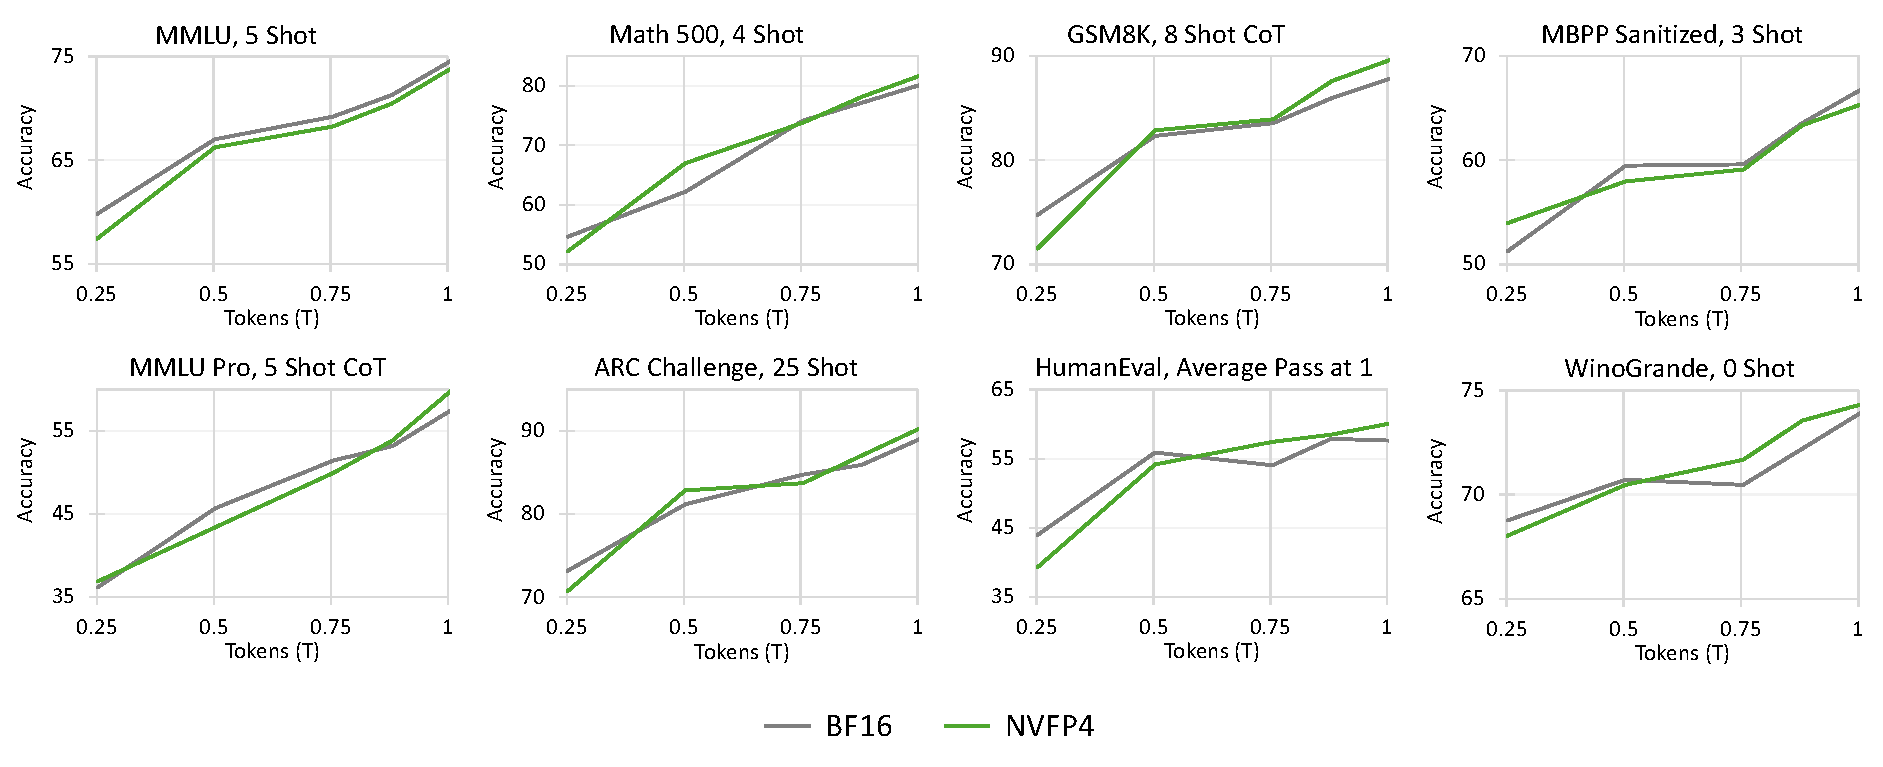
\includegraphics[width=\textwidth]{figures/task_eval_nvfp4.pdf}
    \caption{Downstream task evaluations on 8B active MoE model, trained to 1T tokens. NVFP4 accuracy closely follows BF16 trajectories throughout training. Evaluations are performed in BF16.
    }
    \label{fig:evals_nvfp4_8b}
\end{figure}

Figure~\ref{fig:nanov3_loss_diff_nvfp4} also shows relative loss gaps between NVFP4 and BF16. On Nano, we achieve a < 1\% relative difference in loss between NVFP4 vs BF16 (green). The loss gap decreases to < 0.6\% between NVFP4 vs BF16 when trained on a larger MoE model with 8B active parameters (dark blue). Prior art further reinforces these findings that loss gaps induced from quantization decrease as model size increase ~\citep{chen2025scalinglawquantizationawaretraining}. Downstream task evaluations shown in Figure~\ref{fig:evals_nvfp4_8b} are comparable between the A8B model trained in BF16 vs NVFP4. This phenomenon further confirms prior work on Mamba-MLP models where a small loss gap does not lead to degraded evaluation accuracy ~\citep{nvidia2025pretraininglargelanguagemodels}.
